\section{Computing time bounds}

In this chapter we will present the method, which is able to infer time bounds for transitions of a program.
The original KoAT paper \cite{koat} presented two approaches: One basic approach, considering all transitions and a modular approach, considering a selected subset of transitions.
This master's thesis only considers the modular approach, since the other approach can just be defined as a special case of the modular approach, where the subset of transitions is the set of non-initial transitions $\TSet \setminus \TSet_0$.
The basis of the method are polynomial ranking functions.
The original KoAT allows the usage of arbitrary polynomial ranking functions.
But to obtain monotonicity, it uses an operator which considers the absolute values of variables and converts all negative signs in positive signs.
This is necessary to ensure, that a substitution of the variables with upper size bounds is still a sound overapproximation.
The new method only considers affine ranking functions, but does not need to apply such an operator.
Instead, the signs of the coefficients are considered and the appropriate upper or lower size bound is chosen respectively.
Note that the restriction to affine ranking functions is in practice not a major restriction, since most existing techniques also only generate affine ranking functions (e.g. \cite{podelski2004prf}, \cite{bradley2005linear}, \cite{bagnara2012new}, \cite{leike2014ranking}, \cite{ben2013linear}).

For the definition of the method we need to define the terms of entry locations and entry transitions.
We define the entry locations of a transition set $\TSet' \subseteq \TSet$ as $\mathcal{E}_{\TSet'} = \braced{\location_{in} \mid \TSet_{\location_{in}} \neq \emptyset \wedge \exists \location': (\location_{in}, \update, \guard, \location') \in \TSet'}$.
The entry transitions of a location $\location \in \mathcal{E}_{\TSet'}$ are defined as $\TSet_{\location} = \braced{(\location', \update, \guard, \location) \mid \exists \location', \update, \guard: (\location', \update, \guard, \location) \in \TSet \setminus \TSet'}$.
This is the same definition as used by the original KoAT \cite{koat}.

\begin{figure}
\centering
\begin{tikzpicture}[->,>=stealth',auto,node distance=3cm,
    thick,
    main node/.style={circle,draw,font=\sffamily\Large\bfseries},
    aligned edge/.style={align=left}]

  \node[main node] (0) {$l_0$};
  \node[main node] (1) [right of=0] {$l_1$};
  \node[main node] (2) [right of=1] {$l_2$};
  \node[main node] (3) [right of=2] {$l_3$};

  \path[every node/.style={font=\sffamily\small}]
    (0) edge[aligned edge] node[above=0.2cm] {$t_0$} (1)
    (1) edge[aligned edge, loop above] node[above=0.2cm] {$t_1$} (1)
    (1) edge[aligned edge] node[above=0.2cm] {$t_2$} (2)
    (2) edge[aligned edge, bend left] node[above=0.2cm] {$t_3$} (3)
    (3) edge[aligned edge, bend left] node[below=0.2cm] {$t_4$} (2)
    ;
\end{tikzpicture}
\begin{tikzpicture}[->,>=stealth',auto,node distance=3cm,
    thick,
    main node/.style={circle,draw,font=\sffamily\Large\bfseries},
    aligned edge/.style={align=left}]

  \node[main node] (0) {$l_0$};
  \node[main node, dotted] (1) [right of=0] {$l_1$};
  \node[main node, dotted] (2) [right of=1] {$l_2$};
  \node[main node] (3) [right of=2] {$l_3$};

  \path[every node/.style={font=\sffamily\small}]
    (0) edge[aligned edge] node[above=0.2cm] {$t_0$} (1)
    (1) edge[aligned edge, ultra thick, loop above] node[above=0.2cm] {$t_1$} (1)
    (1) edge[aligned edge] node[above=0.2cm] {$t_2$} (2)
    (2) edge[aligned edge, ultra thick, bend left] node[above=0.2cm] {$t_3$} (3)
    (3) edge[aligned edge, ultra thick, bend left] node[below=0.2cm] {$t_4$} (2)
    ;
\end{tikzpicture}
\caption{A program for showing the difficulties of chosing the right subset of transitions}
\label{fig:entrytransitions}
\end{figure}


As an example, consider the programs in figure \ref{fig:entrytransitions}.
In each of the programs, a chosen set $\TSet' \subseteq \TSet$ is highlighted.
Additionally, all entry locations and entry transitions are shown.
In the first program, the set of transitions $\TSet' = \braced{t_1, t_3, t_4}$ does have two entry locations $\mathcal{E}_{\TSet'} = \braced{\location_1, \location_2}$.
These entry locations define the entry transitions $\TSet_{\location_1} = \braced{t_0}$ and $\TSet_{\location_2} = \braced{t_2}$.
The second program only has one entry location $\mathcal{E}_{\TSet'} = \braced{\location_1}$ and therefore only one entry transition $\TSet_{\location_1} = \braced{t_0}$.
The third program also only has one entry location, but in this example it is $\mathcal{E}_{\TSet'} = \braced{\location_2}$.
Its entry transition is $\TSet_{\location_2} = \braced{t_2}$.

Now it is possible to define the method for the construction of time bounds.

\begin{theorem}[TimeBounds]
  Let $(\UTime, \Size)$ be a complexity approximation. \\
  Let $\TSet' \subseteq \TSet \setminus \TSet_0$ a subset of all transitions such that $\TSet'$ contains no initial transitions. \\
  Let $\TSet_{\location} = \braced{(\location', \update, \guard, \location) \mid \exists \location', \update, \guard: (\location', \update, \guard, \location) \in \TSet \setminus \TSet'}$ denote the set of all transitions outside of the subprogram $\TSet'$ leading to an $\location \in \LSet$. \\
  Let $\mathcal{E}_{\TSet'} = \braced{\location_{in} \mid \TSet_{\location_{in}} \neq \emptyset \wedge \exists \location': (\location_{in}, \update, \guard, \location') \in \TSet'}$ denote the set of all entry locations of $\TSet'$. \\
  Let $\timerank: \LSet \rightarrow \BoundSet_a(\PVSet)$ be an \textbf{affine} time ranking function for $\TSet'$. \\
  For $t \in \TSet'_>$ let
  \[ \UTime'(t) = \sum_{\location \in \mathcal{E}_{\TSet'}} \sum_{\pret \in \TSet_\location} \UTime(\pret) \cdot \maxO{\usubst{\timerank(\location)}{\LSize(\pret)}{\USize(\pret)}} \]
  Let $\UTime'(t) = \UTime(t)$ for $t \in \TSet \setminus \TSet'_>$. \\
  Then, $\text{TimeBounds}(\UTime, (\USize, \LSize), \TSet') = \UTime'$ is also a runtime approximation.
\end{theorem}


The idea of this method is, that with a rank $\timerank(\location)$ for an entry location $\location \in \mathcal{E}_{\TSet'}$ we have a time bound for all decreasing transitions $t \in \TSet'_>$ from the location $\location$.
Then, we need to lift this time bound into a global context, such that it expresses a time bound depending on the variables from the start of the program.
For this purpose, we first need to substitute all variables of the rank $\timerank(\location)$ with the size bounds $\USize(r), \LSize(r)$ from the start to the transition $r \in \TSet_{\location}$ immediately before the location $\location$.
Since $\timerank(\location)$ is affine, it only consists of monotonous variables.
Therefore, the substitution is defined.
Because a time bound can only be positive, we apply to the result $\apprsubst{\timerank(\location)}{\LSize(r)}{\USize(r)}$ a $\maxO{\dot}$ operator.
Now, we have to overapproximate the number of evaluations which might enter through the entry location $\location$.
The previous time bound $\UTime$ yields such a bound for all entry transitions.
Then, $\sum_{\location \in \mathcal{E}_{\TSet'}} \sum_{\pret \in \TSet_\location} \UTime(\pret) \cdot \maxO{\apprsubst{\timerank(\location)}{\LSize(\pret)}{\USize(\pret)}}$ is a time bound for $t \in \TSet'_>$ depending on the variables from the start.

\begin{figure}
  \centering
  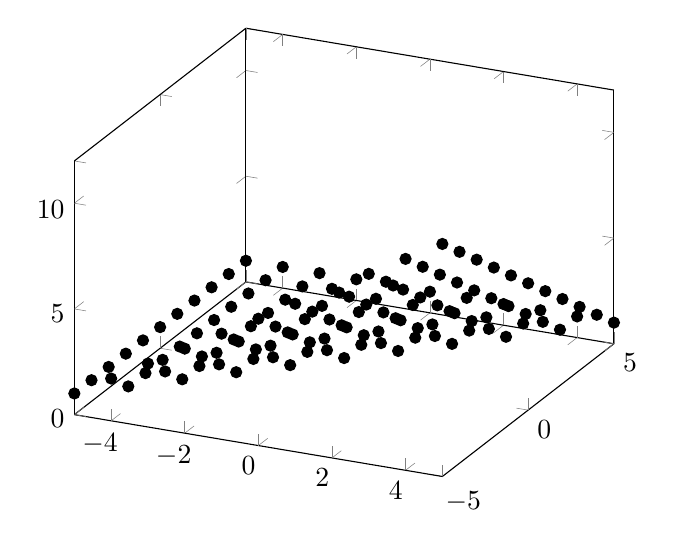
\begin{tikzpicture}
    \begin{axis}
      \addplot3 [
        unbounded coords=jump,
        mesh,
        shader=interp,
        samples at={-5,...,5},
        samples y={11},
        only marks,
      ] {1+max(x-y,0)};
    \end{axis}
  \end{tikzpicture}
  \hfil
  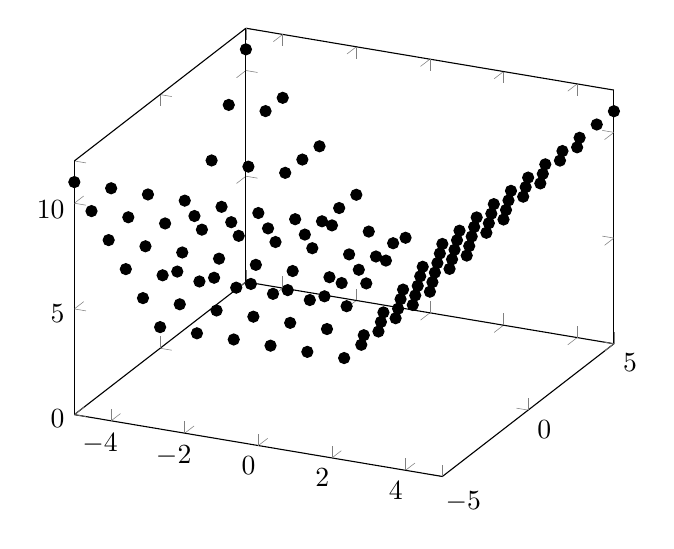
\begin{tikzpicture}
    \begin{axis}
      \addplot3 [
        unbounded coords=jump,
        mesh,
        shader=interp,
        samples at={-5,...,5},
        samples y={11},
        only marks,
      ] {1+abs(max(x,-y))+abs(max(x,-y))};
    \end{axis}
  \end{tikzpicture}
  \caption{Evaluation of the motivational example}
  \label{fig:motivational_evaluation}
\end{figure}


As an example, we consider the motivational program from the introduction \ref{fig:motivational_example}.
With the transition set $\TSet' = \braced{t_1}$ it is possible to determine a ranking function $\timerank(\location_1) = x - y$, since the transition $t_1$ decreases the measure and no transition increases the measure (since no other transition exists in $\TSet'$).
The original KoAT would now apply an operator to $\timerank$, such that the result would be a monotonic function with $\timerank'(\location_1) = \abs{x} + \abs{y}$.
Then it is able to substitute each variable by its absolute size bound and therefore lift it to a global context.
The new method does not use such an operator.
Instead, it substitutes each variable of $\timerank$ by its lower/upper size bound depending on the monotonicity of this component.
Since $x$ is monotonically increasing in $x-y$ and $y$ is monotonically decreasing in $x-y$, we can substitute $x$ with the upper size bound and $y$ with the lower size bound.
Lets assume, that we already inferred the size bounds $\USize(t_0,x) = \LSize(t_0,x) = x$ and $\USize(t_0,y) = \LSize(t_0,y) = y$.
It is now possible to lift the components of the ranking functions to a global level.
\[ \apprsubst{\timerank(\location)}{\LSize(t_0)}{\USize(t_0)} = \USize(t_0, x) - \LSize(t_0, y) = x - y \]
Since with a state $\valuation$ with $\valuation(x) < \valuation(y)$ the transition $t_1$ will simply not occur in an evaluation instead of occurring a negative number of times, we have to ensure the positivity of $x - y$ with the operation $\maxO{x - y}$.
Then, the only step left is to consider the number of times an evaluation might enter the SCC from $t_0$.
Since $t_0$ is an initial transition, its time bound is $\UTime(t_0) = 1$.
Therefore an evaluation might only enter a single time from $t_0$ and the resulting time bound for $t_1$ is $\maxO{x - y}$.

\subsection{Choosing the transition set $\TSet'$}

The choice of the transition set $\TSet'$ has a major impact on the quality of the time bounds.
Consider again the program in figure \ref{fig:entrytransitions} with arbitrary guards and update for each transition.

A trivial approach would be the usage of the second $\TSet'$ with $\TSet' = \TSet \setminus \TSet_0 = \braced{t_1, t_2, t_3, t_4}$.
Then, we have $\mathcal{E}_{\TSet'} = \braced{\location_1}$ and $\TSet_{\location_1} = \braced{t_0}$.
Therefore for each $t \in \TSet'_>$ we end up with $\UTime'(t) = \UTime(t_0) \cdot \maxO{\apprsubst{\timerank(\location_1)}{\LSize(t_0)}{\USize(t_0)}}$.
Since $t_0 \in \TSet_0$ is an initial transition, we have $\UTime(t_0) = 1$ and $\UTime'(t)$ then reflects the expected result of a non-modular approach.

This trivial approach requires us to find a ranking function, that satisfies the non-increasing constraint for all transitions.
If no such ranking function can be found, it is not possible to infer any time bounds with this transition set $\TSet'$.
But since the method allows us to only consider a subset of the transitions, it might be possible, to remove the transition which violates its non-increasing constraint.
Then, a ranking function could be found.

Let's assume that the transition violating the non-increasing constraint is $t_1$ and consider the third example in figure \ref{fig:entrytransitions} with the transition set $\TSet' = \braced{t_3, t_4}$.
Since we reduced the set, we have fewer constraints and are more likely to find a ranking function.
We have $\mathcal{E}_{\TSet'} = \braced{\location_2}$ and $\TSet_{\location_2} = \braced{t_2}$.
Since $t_2$ is not part of a loop, its time bound is $\UTime(t_2) = 1$.
Therefore, we end up with $\UTime'(t) = \maxO{\apprsubst{\timerank(\location_2)}{\LSize(t_2)}{\USize(t_2)}}$.

Note that it is possible to select arbitrary subsets $\TSet' \subseteq \TSet$.
A non-connected subset $\TSet' = \braced{t_1, t_3, t_4}$ could be chosen, but would lead to a bound $\UTime'(t) = \maxO{\apprsubst{\timerank(\location_1)}{\LSize(t_0)}{\USize(t_0)}} + \maxO{\apprsubst{\timerank(\location_2)}{\LSize(t_2)}{\USize(t_2)}}$.
Also only a part of an SCC such as $\TSet' = \braced{t_4}$ could be chosen.
But since $t_3 \in \TSet_{\location_3}$ would be a entry transition of $\TSet' = \braced{t_4}$, this would only be of benefit if we already inferred a time bound $\UTime(t_3) < \infty$.

The implementation selects the transitions of the different SCCs of the program as transition set $\TSet'$ and excludes those transitions $t$, for which we already inferred a time bound $\UTime(t) < \infty$.
